% Copyright 2007 by Till Tantau and Mark Wibrow
%
% This file may be distributed and/or modified
%
% 1. under the LaTeX Project Public License and/or
% 2. under the GNU Free Documentation License.
%
% See the file doc/generic/pgf/licenses/LICENSE for more details.


\section{Shadows Library}
\label{section-libs-shadows}

\begin{tikzlibrary}{shadows}
    This library defines styles that help adding a (partly) transparent shadow
    to a path or node.
\end{tikzlibrary}
%
\begin{codeexample}[setup code,hidden]
    \usetikzlibrary{shadows}
\end{codeexample}


\subsection{Overview}

A \emph{shadow} is usually a black or gray area that is drawn behind a path or
a node, thereby adding visual depth to a picture. The |shadows| library defines
options that make it easy to add shadows to paths. Internally, these options
are based on using the |preaction| option to use a path twice: Once for drawing
the shadow (slightly shifted) and once for actually using the path.

Note that you can only add shadows to \emph{paths}, not to whole scopes.

In addition to the general |shadow| option, there exist special options like
|circular shadow|. These can only (sensibly) be used with a special kind of
path (for |circular shadow|, a circle) and, thus, they are not as general. The
advantage is, however, that they are more visually pleasing since these shadows
blend smoothly with the background. Note that these special shadows use
fadings, which few printers will support.


\subsection{The General Shadow Option}

The shadows are internally created by using a single option called
|general shadow|. The different options like |drop shadow| or |copy shadow|
only differ in the commands that they preset.

You will not need to use this option directly under normal circumstances.

\begin{key}{/tikz/general shadow=\meta{shadow options} (default \normalfont empty)}
    This option should be given to a |\path| or a |node|. It has the following
    effect: Before the path is used normally, it is used once with the
    \meta{shadow options} in force. Furthermore, when the path is ``preused''
    in this way, it is shifted and scaled a little bit.

    In detail, the following happens: A |preaction| is used to paint the path
    in a special manner before it is actually painted. This ``special'' manner
    is as follows: The options in \meta{shadow options} are used for painting
    this path. Typically, the \meta{shadow options} will contain options like
    |fill=black| to create, say, a black shadow. Furthermore, after the
    \meta{shadow options} have been set up, the following extra canvas
    transformations are applied to the path: It is scaled by |shadow scale|
    (with the origin of scaling at the path's center) and it is shifted by
    |shadow xshift| and |shadow yshift|.

    Note that since scaling and shifting is done using canvas transformations,
    shadows are not taken into account when the picture's bounding box is
    computed.
    %
\begin{codeexample}[]
\tikz [even odd rule]
  \draw [general shadow={fill=red}] (0,0) circle (.5) (0.5,0) circle (.5);
\end{codeexample}

    \begin{key}{/tikz/shadow scale=\meta{factor} (initially 1)}
        Shadows are scaled by \meta{factor}.
        %
\begin{codeexample}[]
\tikz [even odd rule]
  \draw [general shadow={fill=red,shadow scale=1.25}]
    (0,0) circle (.5) (0.5,0) circle (.5);
\end{codeexample}
    \end{key}
    %
    \begin{key}{/tikz/shadow xshift=\meta{dimension} (initially 0pt)}
        Shadows are shifted horizontally by \meta{dimension}.
        %
\begin{codeexample}[]
\tikz [even odd rule]
  \draw [general shadow={fill=red,shadow xshift=-5pt}]
    (0,0) circle (.5) (0.5,0) circle (.5);
\end{codeexample}
    \end{key}
    %
    \begin{key}{/tikz/shadow yshift=\meta{dimension} (initially 0pt)}
        Shadows are shifted vertically by \meta{dimension}.
    \end{key}
\end{key}


\subsection{Shadows for Arbitrary Paths and Shapes}

\subsubsection{Drop Shadows}

\begin{key}{/tikz/drop shadow=\meta{shadow options} (default \normalfont empty)}
    This option adds a drop shadow to a |\path| or a |node|. It uses the
    |general shadow| and passes the \meta{shadow options} to it, plus, before
    them, the following extra options:
    %
\begin{codeexample}[code only]
  shadow scale=1, shadow xshift=.5ex, shadow yshift=-.5ex,
  opacity=.5, fill=black!50, every shadow
\end{codeexample}

\begin{codeexample}[]
\tikz [even odd rule]
  \filldraw [drop shadow,fill=white] (0,0) circle (.5) (0.5,0) circle (.5);
\end{codeexample}

\begin{codeexample}[preamble={\usetikzlibrary{shapes.symbols}}]
\begin{tikzpicture}
  \foreach \i in {1,...,4}
    \node[starburst,drop shadow,fill=white,draw] at (0,\i) {Burst \i};
\end{tikzpicture}
\end{codeexample}

\begin{codeexample}[]
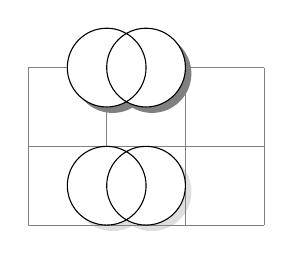
\begin{tikzpicture}
  \draw [help lines] (0,0) grid (3,2);
  \filldraw [drop shadow={opacity=1},fill=white]
    (1,2)  circle (.5) (1.5,2)  circle (.5);

  \filldraw [drop shadow={opacity=0.25},fill=white]
    (1,.5) circle (.5) (1.5,.5) circle (.5);
\end{tikzpicture}
\end{codeexample}
    %
\end{key}

\begin{stylekey}{/tikz/every shadow (initially \normalfont empty)}
    This style is executed in addition to any \meta{shadow options} for each
    shadow. Use this style to reconfigure the way shadows are drawn.
    %
\begin{codeexample}[]
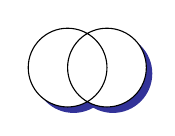
\begin{tikzpicture}[every shadow/.style={opacity=.8,fill=blue!50!black}]
  \filldraw [drop shadow,fill=white] (0,0) circle (.5) (0.5,0) circle (.5);
\end{tikzpicture}
\end{codeexample}
    %
\end{stylekey}


\subsubsection{Copy Shadows}

A \emph{copy shadow} is not really a shadow. Rather, it looks like another copy
of the path drawn behind the path and a little bit offset. This creates the
visual impression of having multiple copies of the path/object present.

\begin{key}{/tikz/copy shadow=\meta{shadow options} (default \normalfont empty)}
    This shadow installs the following default options:
    %
\begin{codeexample}[code only]
  shadow scale=1, shadow xshift=.5ex, shadow yshift=-.5ex, every shadow
\end{codeexample}
    %
    Furthermore, the options |fill=|\meta{fill color} and |draw=|\meta{draw
    color} are also set, where the \meta{fill color} and \meta{draw color} are
    the fill and draw colors used for the main path.
    %
\begin{codeexample}[preamble={\usetikzlibrary{shapes.symbols}}]
\begin{tikzpicture}
  \node [copy shadow,fill=blue!20,draw=blue,thick] {Hello World!};

  \node at (0,-1) [copy shadow={shadow xshift=1ex,shadow yshift=1ex},
                   fill=blue!20,draw=blue,thick]
    {Hello World!};

  \node at (0,-2) [copy shadow={opacity=.5},tape,
                   fill=blue!20,draw=blue,thick]
    {Hello World!};

  % We have to repeat the left color since shadings are not
  % automatically applied to shadows
  \node at (0,-3) [copy shadow={left color=blue!50},
                   left color=blue!50,draw=blue,thick]
    {Hello World!};
\end{tikzpicture}
\end{codeexample}
    %
\end{key}

\begin{key}{/tikz/double copy shadow=\meta{shadow options} (default \normalfont empty)}
    This shadow works like a |copy shadow|, only the shadow is added twice, the
    second time with the double |xshift| and |yshift|.
    %
\begin{codeexample}[preamble={\usetikzlibrary{shapes.symbols}}]
\begin{tikzpicture}
  \node [double copy shadow,fill=blue!20,draw=blue,thick] {Hello World!};

  \node at (0,-1) [double copy shadow={shadow xshift=1ex,shadow yshift=1ex},
                   fill=blue!20,draw=blue,thick]
    {Hello World!};

  \node at (0,-2) [double copy shadow={opacity=.5},tape,
                   fill=blue!20,draw=blue,thick]
    {Hello World!};

  \node at (0,-3) [double copy shadow={left color=blue!50},
                   left color=blue!50,draw=blue,thick]
    {Hello World!};
\end{tikzpicture}
\end{codeexample}
    %
\end{key}


\subsection{Shadows for Special Paths and Nodes}

The shadows in this section should normally be added only to paths that have a
special shape. They will look strange with other shapes.

\begin{key}{/tikz/circular drop shadow=\meta{shadow options}}
    This shadow works like a drop shadow, only it adds a circular fading to the
    shadow. This means that the shadow will fade out at the border. The
    following options are preset for this shadow:
    %
\begin{codeexample}[code only]
  shadow scale=1.1, shadow xshift=.3ex, shadow yshift=-.3ex,
  fill=black, path fading={circle with fuzzy edge 15 percent},
  every shadow,
\end{codeexample}

\begin{codeexample}[]
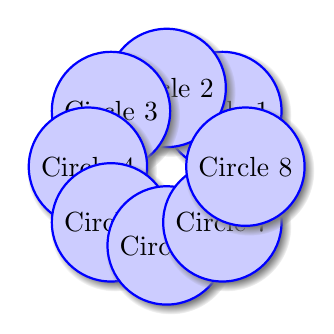
\begin{tikzpicture}
  \foreach \i in {1,...,8}
    \node[circle,circular drop shadow,draw=blue,fill=blue!20,thick]
      at (\i*45:1) {Circle \i};
\end{tikzpicture}
\end{codeexample}
    %
\end{key}

\begin{key}{/tikz/circular glow=\meta{shadow options}}
    This shadow works much like the |circular shadow|, only it is not shifted.
    This creates a visual effect of a ``glow'' behind the circle. The following
    options are preset for this shadow:
    %
\begin{codeexample}[code only]
  shadow scale=1.25, shadow xshift=0pt, shadow yshift=0pt,
  fill=black, path fading={circle with fuzzy edge 15 percent},
  every shadow,
\end{codeexample}

\begin{codeexample}[]
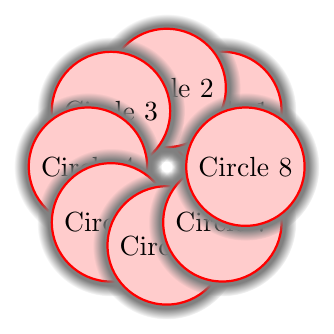
\begin{tikzpicture}
  \foreach \i in {1,...,8}
  \node[circle,circular glow,fill=red!20,draw=red,thick]
    at (\i*45:1) {Circle \i};
\end{tikzpicture}
\end{codeexample}

\begin{codeexample}[]
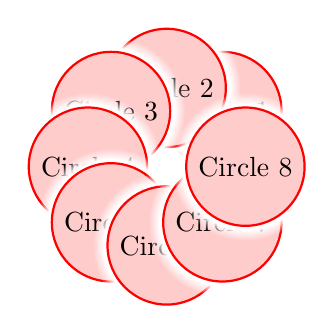
\begin{tikzpicture}
  \foreach \i in {1,...,8}
  \node[circle,circular glow={fill=white},fill=red!20,draw=red,thick]
    at (\i*45:1) {Circle \i};
\end{tikzpicture}
\end{codeexample}

\begin{codeexample}[]
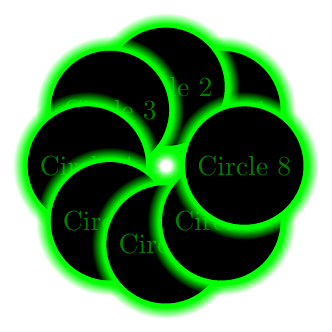
\begin{tikzpicture}
  \foreach \i in {1,...,8}
  \node[circle,circular glow={fill=green},fill=black,text=green!50!black]
    at (\i*45:1) {Circle \i};
\end{tikzpicture}
\end{codeexample}
    %
    An especially interesting effect can be achieved by only using the glow and
    not filling the path:
    %
\begin{codeexample}[]
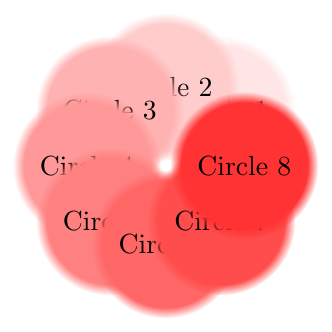
\begin{tikzpicture}
  \foreach \i in {1,...,8}
  \node[circle,circular glow={fill=red!\i0}]
    at (\i*45:1) {Circle \i};
\end{tikzpicture}
\end{codeexample}
    %
\end{key}


%%% Local Variables:
%%% mode: latex
%%% TeX-master: "pgfmanual-pdftex-version"
%%% End:
